\documentclass[french]{scrartcl}
\usepackage[T1]{fontenc}
\usepackage[utf8]{inputenc}
\usepackage{lmodern}
\usepackage[a4paper]{geometry}
\usepackage{subcaption}
\usepackage{graphicx}
\usepackage{listings}
\usepackage{xcolor}
\usepackage{hyperref}
\usepackage{babel}

\hypersetup{
	colorlinks,
	citecolor=black,
	filecolor=black,
	linkcolor=black,
	urlcolor=black
}

\definecolor{pblue}{rgb}{0.13,0.13,1}
\definecolor{pgreen}{rgb}{0,0.5,0}
\definecolor{pred}{rgb}{0.9,0,0}
\definecolor{pgrey}{rgb}{0.46,0.45,0.48}

\lstset{language=Java,
	showspaces=false,
	showtabs=false,
	breaklines=true,
	showstringspaces=false,
	breakatwhitespace=true,
	commentstyle=\color{pgreen},
	keywordstyle=\color{pblue},
	stringstyle=\color{pred},
	basicstyle=\ttfamily,
	tabsize=2,
	numbers=left
}

% Commands

\newcommand{\fx}{\emph{JavaFX} }
\newcommand{\java}{\emph{Java} }
\newcommand{\himalaya}{\emph{Himalaya} }
\newcommand{\reference}[1]{(Voir Figure \ref{fig:#1},  page \pageref{fig:#1}) }

% Begin document

\begin{document}
	
% Title Page
\begin{titlepage}
	\begin{center}
		\vspace*{2cm}
		
		\Huge
		\textbf{Himalaya}
		
		\line(1,0){200}
		
		\vspace{0.5cm}
		\LARGE
		Rapport de projet
		
		\vspace{4.5cm}
		
		\large
		Alexis Jouin \& Sébastien Schouteeten
		
		\vspace{0.5cm}
		Master 1 ISIDIS
		
		\vfill
		
		
\includegraphics[width=0.5\textwidth]{images/ulco}
		
		\vspace{0.8cm}
		
		\Large
		Années 2016 - 2017
		
	\end{center}
\end{titlepage}

\newpage

\tableofcontents

\newpage

\section{Remerciements}
Nous tenons à remercier notre enseignant tuteur, Monsieur Cyril Fonlupt, pour son aide pour le bon déroulement de notre projet. Remerciements également à monsieur Sébastien Verel et monsieur Fabien Teytaud pour les cours de recherches opérationnels et apprentissage artificiel, qui nous a apporté une aide précieuse pour le bon déroulement du projet.

\newpage

\section{Introduction}
Le projet de fin d'année de Master \emph{ISIDIS} est très intéressant et important pour nous initier à un travail de recherche.
Nous avons fait le choix de travailler sur le projet \himalaya en binôme, ce qui implique tout de même une organisation dans les tâches de travaux.
On a fait ce choix, car nous étions intéressés de développer un bot en \java pour un jeu de société.
De plus, ce projet nous a permis d’utiliser de nouvelles technologies que nous ne maîtrisions pas comme \fx.
Notre binôme est composé Sébastien Schouteeten et Alexis Jouin.
À partir de ce constat, nous avons donc essayé de réaliser un logiciel fonctionnel, remplissant les conditions imposées par le cahier des charges validé par monsieur Fonlupt. Nous allons donc voir à travers ce rapport dans une première partie, une présentation du projet ainsi que ses principaux objectifs. Puis dans une seconde partie, les méthodes que nous avons utilisées afin de mettre en \oe uvre le projet et son élaboration. Enfin, dans la dernière partie, nous verrons les résultats obtenus ainsi que les évolutions possibles du projet et plus particulièrement du logiciel.

\newpage

\section{Étude du projet}
\subsection{Contraintes et situations initiales}
Le projet initial à réaliser est un bot en \java pour le jeu de société \himalaya. Le moteur du jeu a déjà été réalisé par l'Université de Nice. Cependant, pour des raisons techniques et pratiques nous avons dû repartir à zéro afin de construire un moteur de jeu plus adapté pour une interface graphique (avec \fx) et les intelligences artificielles. Nous nous sommes tout de même inspirés du travail réalisé précédemment.

\subsection{Pourquoi \fx ?}
\fx contient des outils et composants graphiques les plus maintenus du langage \java.
De plus, cette <<API>> est très rapide et simple à utiliser.
Cela nous a permis en plus d’apprendre et de maitriser un nouvel outil de développement d’interface graphique en \java.

\subsection{Objectifs à réaliser}
Les objectifs principaux du projet ont été de :
\begin{itemize} 
	\item Construire le moteur du jeu 
	\item Construire l'interface graphique
	\item Construire l’intelligence artificielle du jeu
\end{itemize}


\newpage

\section{Élaboration du projet}

\subsection{Les différentes phases du projet}
	\subsubsection{Création du moteur du jeu}
		
		Nous avons débuté le projet par la création du moteur du jeu.
		Ce moteur a été pensé à l'avance avec la réalisation de l'\emph{UML},
		représentant les classes \java.
		Nous nous sommes également aidés du code source du jeu qui nous a été fourni
		en début de projet.
		
		Le moteur du jeu est réalisé de manière à pouvoir être utilisé aussi bien en
		console (terminal), qu'avec une interface graphique.
		
		Durant la réalisation du moteur, nous avons mis en place des tests unitaires,
		dans le but de pouvoir tester notre code, et vérifier qu'aucune des
		fonctionnalités précédentes n'est altérée par les nouvelles.
		
		Nous avons réalisé une classe \emph{Player.java} qui représente un joueur humain,
		et nous avons créé ses classes filles pour utiliser les intelligences artificielles.
		
	\subsubsection{Création de l'interface}
	
		Une fois le moteur terminé et les tests unitaires finis, nous avons réalisé une interface en console.
		Cette dernière nous a permis de réaliser des tests avec une vraie personne qui joue, et de 
		commencer à mettre en place une intelligence artificielle.
		
		Par la suite, nous avons commencé à travailler sur une interface graphique
		du jeu. Nous avons choisi d'utiliser \fx pour réaliser cette étape, car c'est
		la méthode la plus rapide pour mettre en place une interface fonctionnelle en \java.
		En effet, \fx est maintenant la bibliothèque de création d'interfaces graphiques officielle du langage \java.
		
		Nous avons réalisé un menu \reference{menu}, qui permet de sélectionner les joueurs et leur type (Humain, IA aléatoire ou Évolutionnaire). Il est possible, depuis ce menu, de passer en mode 3 ou 4 joueurs.
		
		Juste avant de pouvoir jouer, le jeu demande aux joueurs de choisir leur position de départ \reference{pos_init}.
		
		Durant le déroulement du jeu, nous affichons le plateau ainsi que les ressources
		possédées pour chaque joueur, ainsi que les commandes et ressources proposées sur
		les villages. Les pions des joueurs ainsi que les délégations et stupas qu'ils ont posés
		apparaissent également sur le plateau de jeu \reference{etat_jeu}.
		
		La sélection des actions est effectuée dans une nouvelle fenêtre \reference{actions}, dans laquelle
		le joueur va pouvoir sélectionner les 6 actions qu'il veut effectuer, ainsi que
		la choix de la région s'il choisit de poser une délégation.
		
		À la fin de la partie, une fenêtre s'ouvre et affiche les scores de chaque joueur
		dans chacun des domaines (Politique, Religieux et Économique), ainsi que le vainqueur \reference{resultats}.
			
	\subsubsection{Création des intelligences artificielles}
	
		Nous avons tout d'abord réalisé une IA aléatoire, dans un but de rapidité et de test.
		En effet, celle-ci nous a permis de réaliser une partie, et de vérifier que les différentes actions 
		s'effectuent correctement. Elle choisit 6 actions de manière aléatoire.
		Cette IA a été utile pour tester l'affichage de l'interface graphique, et sa
		mise à jour durant l'exécution des tours : les actions sont effectuées une
		à une, avec une courte pause entre chaque, pour permettre de bien suivre le déroulement du jeu.
		
		Nous avons ensuite commencé le développement de l'IA basée sur un algorithme évolutionnaire.
		Cette dernière utilise l'algorithme évolutionnaire pour réaliser deux choses différentes:
		\begin{itemize}
			\item Choisir sa position de départ.
			\item Planifier les actions qu'elle va réaliser durant le tour.
		\end{itemize}
		
		L'algorithme va réaliser, pour chaque génération, une suite d'actions:
		\begin{enumerate}
			\item Une sélection: on sélectionne les individus qui vont participer à la reproduction.
			\item Des mutations de la population des enfants: mutation ou crossing-over, suivant un ratio donné.
			\item Évaluer la population des enfants, en calculant leur fitness.
			\item effectuer un remplacement: on garde les meilleurs individus pour composer la nouvelle population de parents.
		\end{enumerate}
		
		\lstinputlisting[language=Java, frame=tb, caption= {Déroulement de l'algorithme évolutionnaire}]{code/algo_evol.java}


\section{L'intelligence artificielle}

\subsection{L'algorithme}
	
	\subsubsection{Les paramètres de l'algorithme}
	
		L'algorithme évolutionnaire utilise plusieurs paramètres durant son exécution.
		Nous avons fait varier ses différents paramètres pour voir leur impact, pour des valeurs plus ou moins importantes,
		sur la fitness généralement obtenue, et les actions effectuées par l'IA.
		
		Nous avons fixé la taille de la population des parents (mu) à 20, pour garder à chaque génération les 20 meilleures
		solutions. Ce paramètre ne doit pas être trop élevé pour éviter les mauvaises solutions d'être prise dans la sélection.
		Il doit également ne pas être trop faible sinon les solutions vont devenir trop diverses.
		
		Concernant la taille de la population des enfants (lambda), nous l'avons fixé à 500, car cela permet de garder une diversité et d'explorer de nouvelles solutions possibles.
		
		Le paramètre suivant est la taille du tournoi pour la sélection. Le nombre ne doit pas être trop élevé sinon
		on risque d'obtenir une nouvelle population d'individus identiques à la population de parents.
		
		Le taux de crossing-over et le taux de mutation sont les paramètres qui vont influer sur les variations
		que va subir la population d'enfants obtenue. Le taux conservé pour le crossing-over est de 80\%, et le taux
		retenu pour la mutation est de 100\%. Le taux de mutation fixé à 100\% permet d'assurer à la population d'enfants
		d'être un minimum différente de la population des parents.
		
		Il reste enfin à déterminer le nombre de générations à effectuer pour une exécution de l'algorithme.
		Le nombre de générations maximum que nous avons retenu est 25, en effet, la fitness n'évolue que très 
		rarement au-delà de la 25\ieme{} génération. De plus, si le nombre de générations est trop élevé, cela
		ralentit grandement l'exécution de l'algorithme.
	
	\subsubsection{Présentation d'une solution}
	
		Une solution est un individu d'une population de l'algorithme. Chacune d'entre elles représente une suite de
		9 actions, l'IA va effectuer les 6 premières actions de la solution durant le tour. En effet, une solution est
		calculée grâce à une simulation du prochain tour à jouer, ainsi que 3 actions supplémentaires. Cela va permettre à
		l'IA d'obtenir la meilleure position de départ possible sur le tour suivant.

\subsection{La fitness}
			
	\subsubsection{Calcul de la fitness}
	
		\vbox{
			\lstinputlisting[language=Java, frame=tb, caption= {Pseudo-code: Calcul de la fitness}]{code/algo_fitness.java}
			
		}
		
		Pour calculer la fitness, une copie du plateau de jeu ainsi que de tous ses composants est faite.
		Uniquement l'IA évolutionnaire est copiée sur le nouveau plateau, les autres joueurs n'y apparaissent pas. Une simulation est alors réalisée: le tour est lancé sur le plateau copié, et la copie de l'IA réalise ses 9 actions. Au bout de 6 actions (un tour normal),
		on ajoute un malus à la fitness si le joueur a honoré une commande mais n'a pas pris 2 récompenses.
		
		Une fois le malus additionné, le restant des actions est réalisé, permettant d'améliorer la position de l'IA à
		la fin du tour, et d'anticiper les actions du prochain tour.
		Anticiper la position de l'IA permet d'éviter que celle-ci ne fasse pas d'action inutile à la fin de son tour,
		par exemple des allers-retours ou s'éloigner des villages intéressants.
		
		La fitness est ensuite calculée sur les différents domaines (politique, religieux et économique), ainsi que sur
		le nombre de ressources ramassées. À chaque domaine calculé est ajouté un coefficient, qui est obtenu en
		comparant le score de l'IA avec celui des autres joueurs. Les coefficients sont égaux pour tous les joueurs en début de partie, ils sont plus élevés dans le ou les domaines ou l'IA perd au niveau du score. Inversement,
		le coefficient va diminuer de moitié si l'IA est en tête dans le domaine correspondant.
		
		Chaque domaine se voit également associer un poids qui permet, pour l'IA, d'avoir une grande amélioration de
		fitness dans le cas où celle-ci réaliserait une commande et ferait augmenter son score dans un ou plusieurs domaines.
		
	\subsubsection{Détermination de la position initiale}
	
		La position initiale de l'IA évolutionnaire est déterminée en réalisant, pour chaque village qui n'est pas
		encore choisi par un joueur, un run de l'algorithme génétique. On considère que le village en cours d'analyse est la position du joueur. La meilleur fitness obtenue est enregistrée. On compare ensuite toutes les fitness
		et on garde la meilleure: le village correspondant à cette meilleur fitness est choisi comme position de départ de l'IA.
			
	\subsubsection{Choix de la région optimale pour les délégations}
	
		Lorsque l'IA choisit d'honorer une commande et d'ensuite poser des délégations, un calcul est réalisé pour déterminer la région qui va lui rapporter le plus de points.
		
		Un calcul de rentabilité est effectué pour chaque région avoisinante, il s'agit de faire la différence entre le nombre de délégations que l'IA peut poser avec le nombre de délégations déjà présentes sur cette région.
		Grâce à ce calcul, l'IA va poser des délégations seulement si une région n'en possède pas, ou si elle peut battre le joueur qui la contrôle.
		

\newpage
\section{Résultats et perspectives}
	\subsection{Résultat final}
	
	\subsection{Améliorations possibles}

\newpage
\section{Conclusion}

\newpage
\section{Annexes}

\begin{figure}[h]
	\centering
	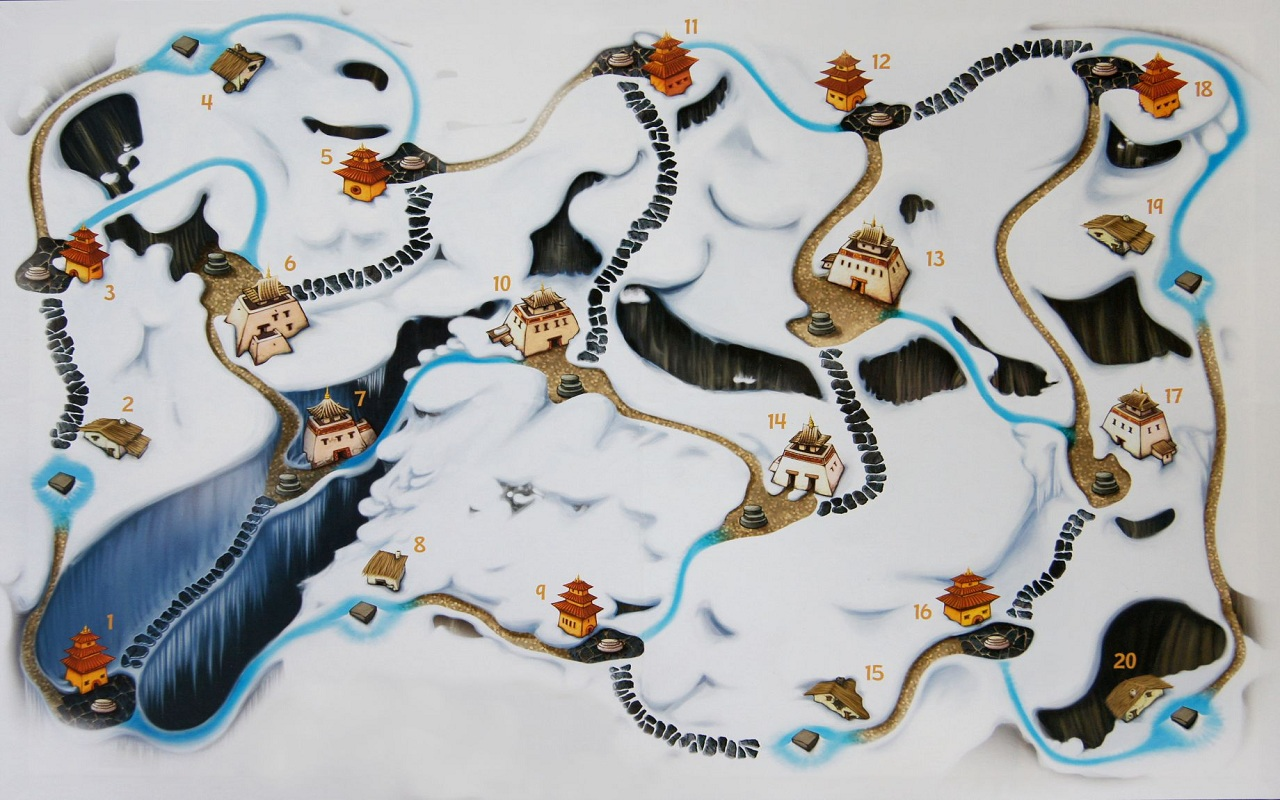
\includegraphics[width=0.7\linewidth]{images/plateau}
	\caption{Plateau du jeu}
	\label{fig:plateau}
\end{figure}

\begin{figure}[h]
	\centering
	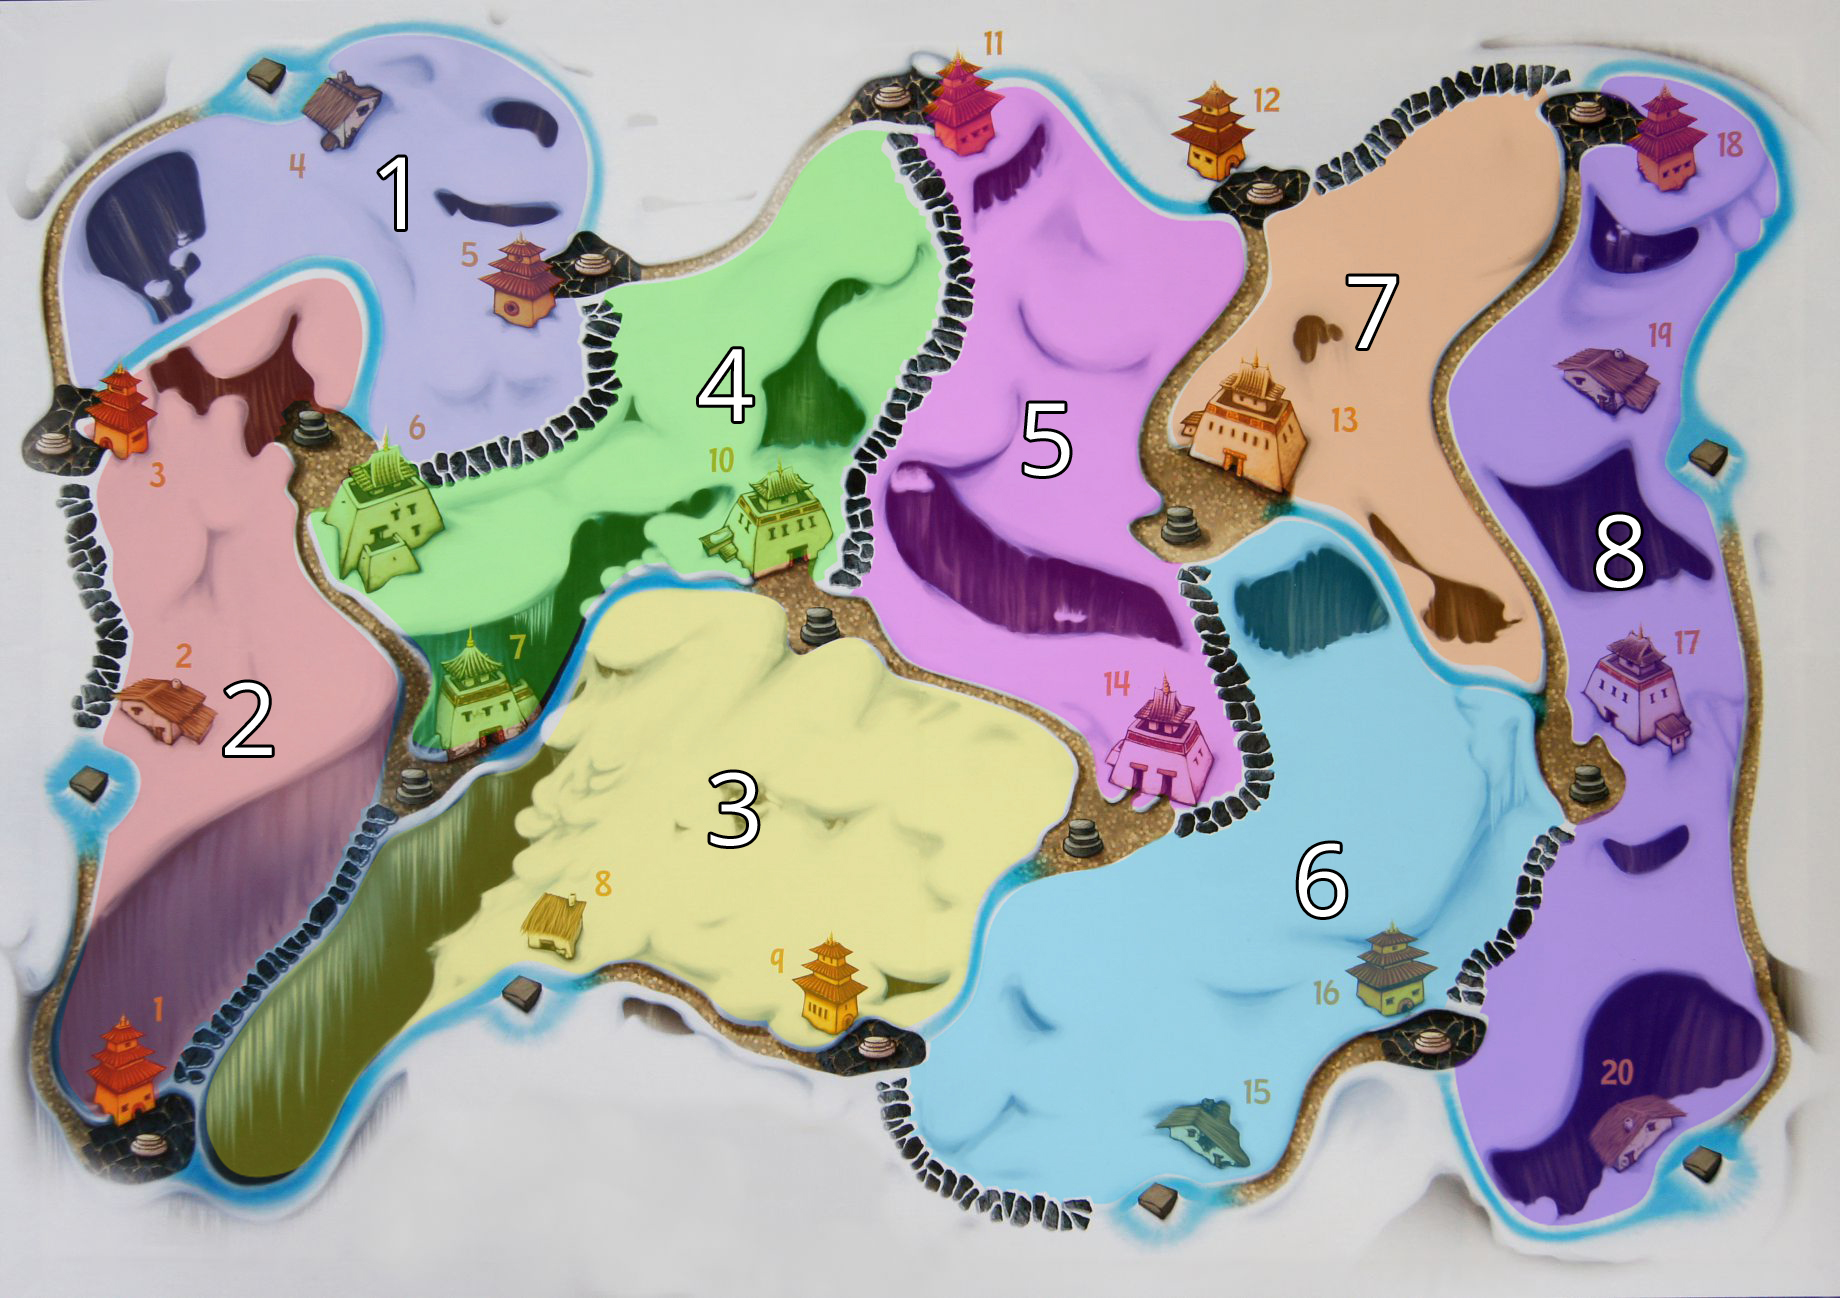
\includegraphics[width=0.7\linewidth]{images/board_regions}
	\caption{Répartitions des régions}
	\label{fig:board_region}
\end{figure}

\begin{figure}[h]
	\centering
	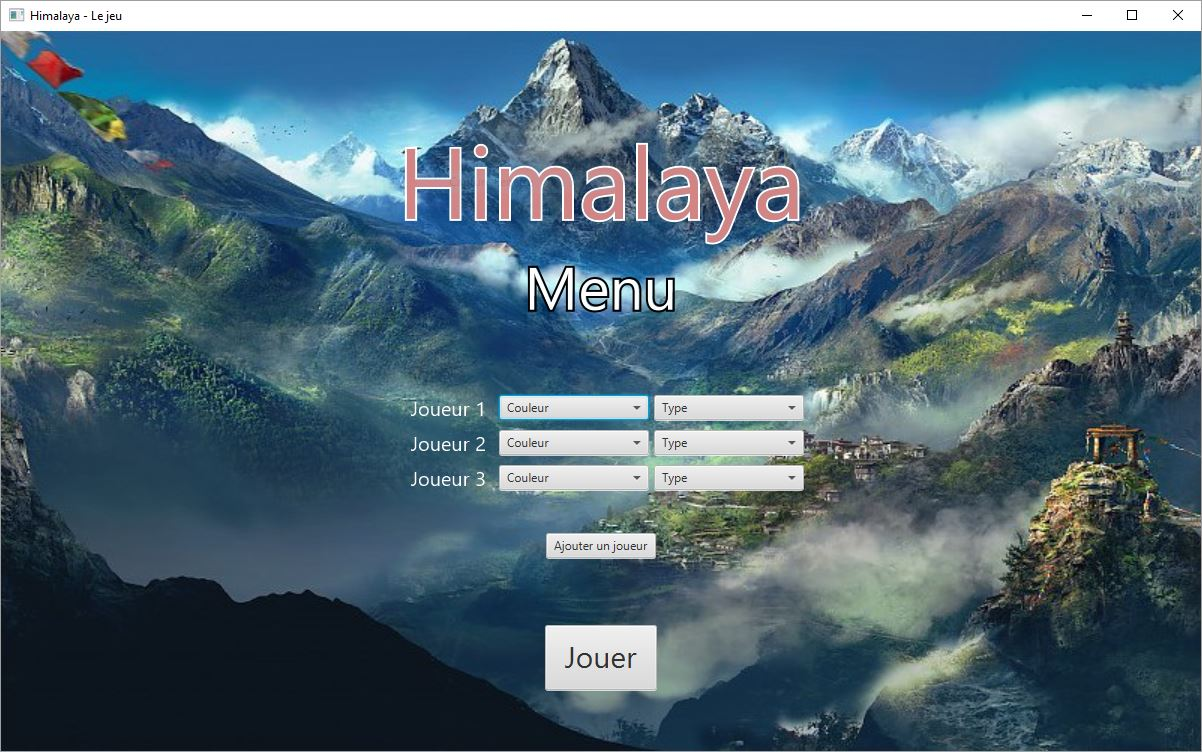
\includegraphics[width=0.9\linewidth]{images/menu}
	\caption{Menu du jeu}
	\label{fig:menu}
\end{figure}

\begin{figure}[h]
	\centering
	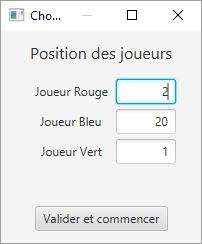
\includegraphics[width=0.4\linewidth]{images/position}
	\caption{Positions initiales}
	\label{fig:pos_init}
\end{figure}

\begin{figure}[h]
	\centering
	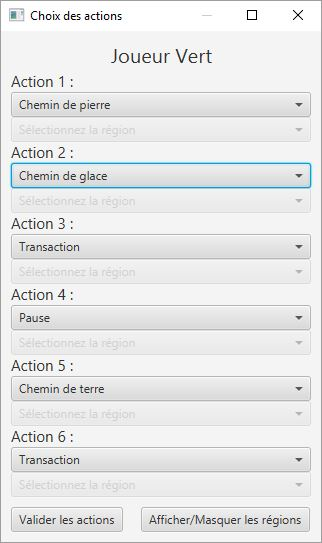
\includegraphics[width=0.4\linewidth]{images/actions}
	\caption{Choix des actions (joueur humain)}
	\label{fig:actions}
\end{figure}

\begin{figure}[h]
	\centering
	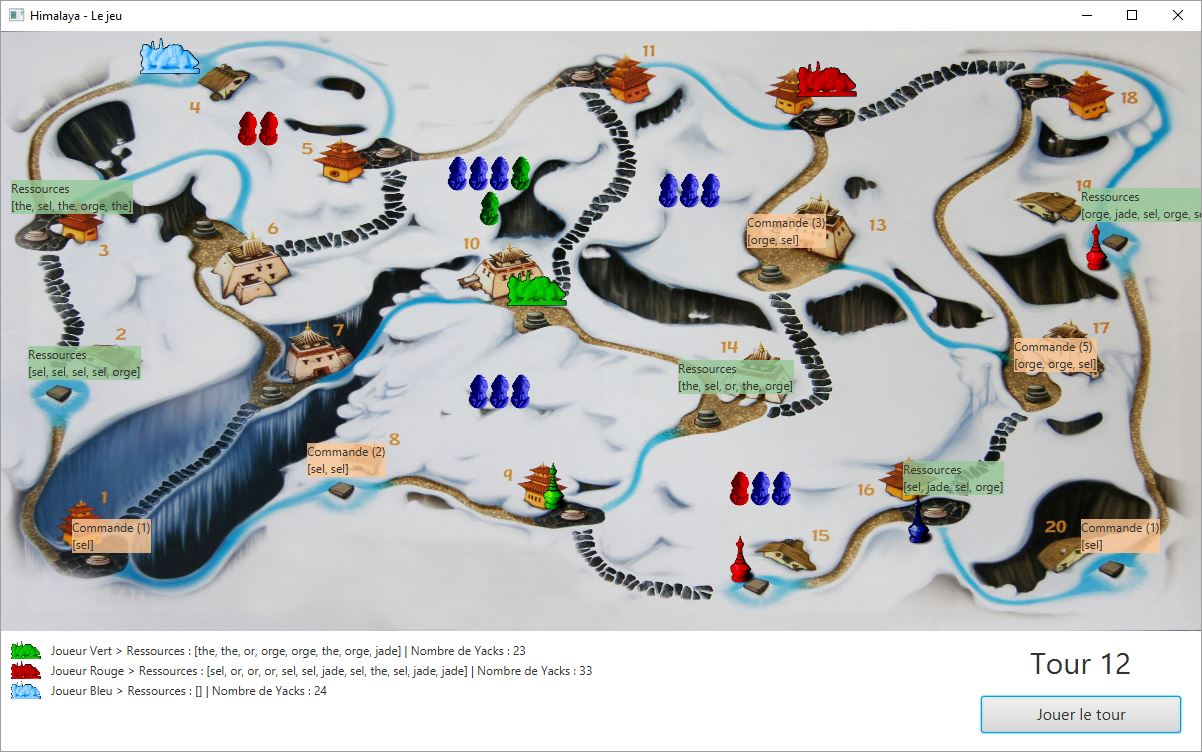
\includegraphics[width=0.9\linewidth]{images/etat_jeu_avance}
	\caption{Déroulement du jeu}
	\label{fig:etat_jeu}
\end{figure}

\begin{figure}[h]
	\centering
	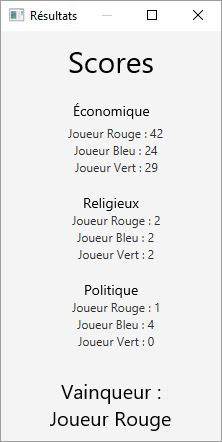
\includegraphics[width=0.3\linewidth]{images/resultats}
	\caption{Résultats de la partie}
	\label{fig:resultats}
\end{figure}

\begin{figure}[h]
	\centering
	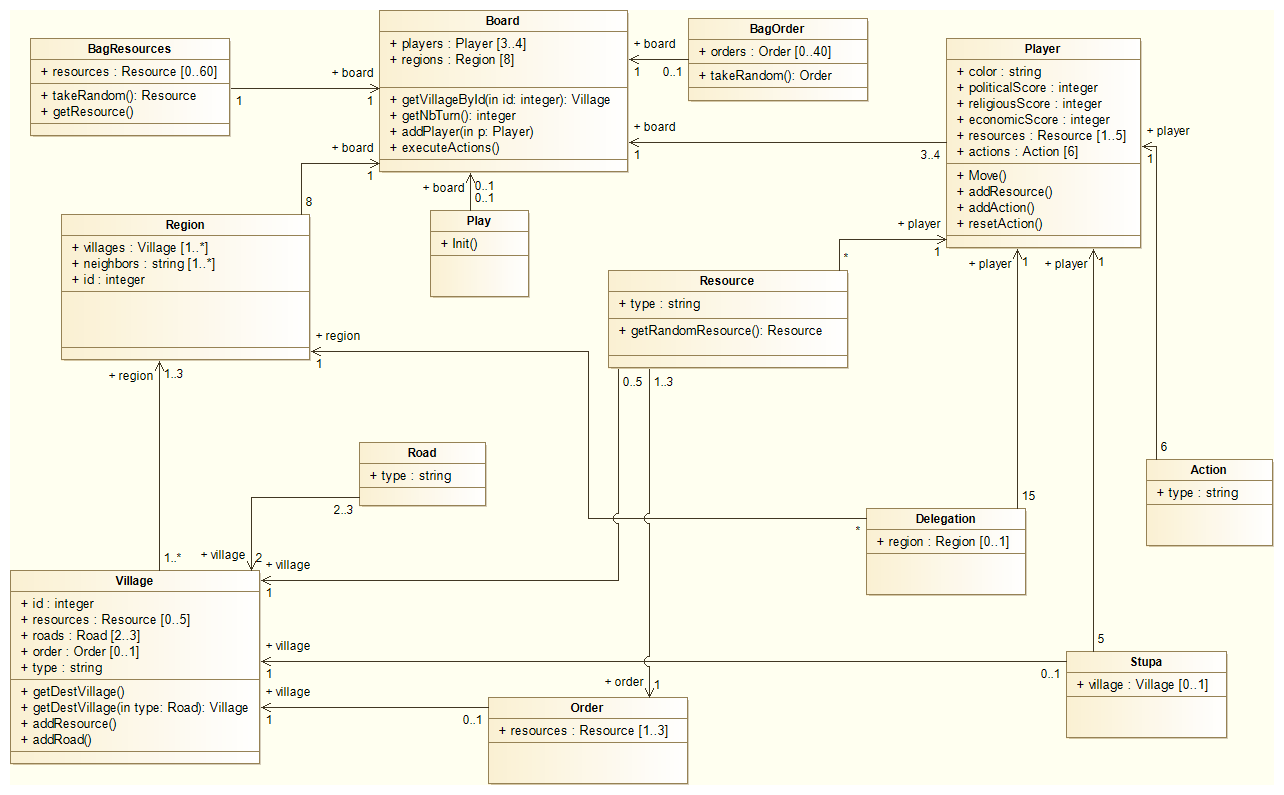
\includegraphics[width=1\linewidth]{images/UML_Himalaya_2}
	\caption{UML Moteur du jeu version 2.5 avant développement}
	\label{fig:UMLCore1}
\end{figure}
\begin{figure}[h]
	\centering
	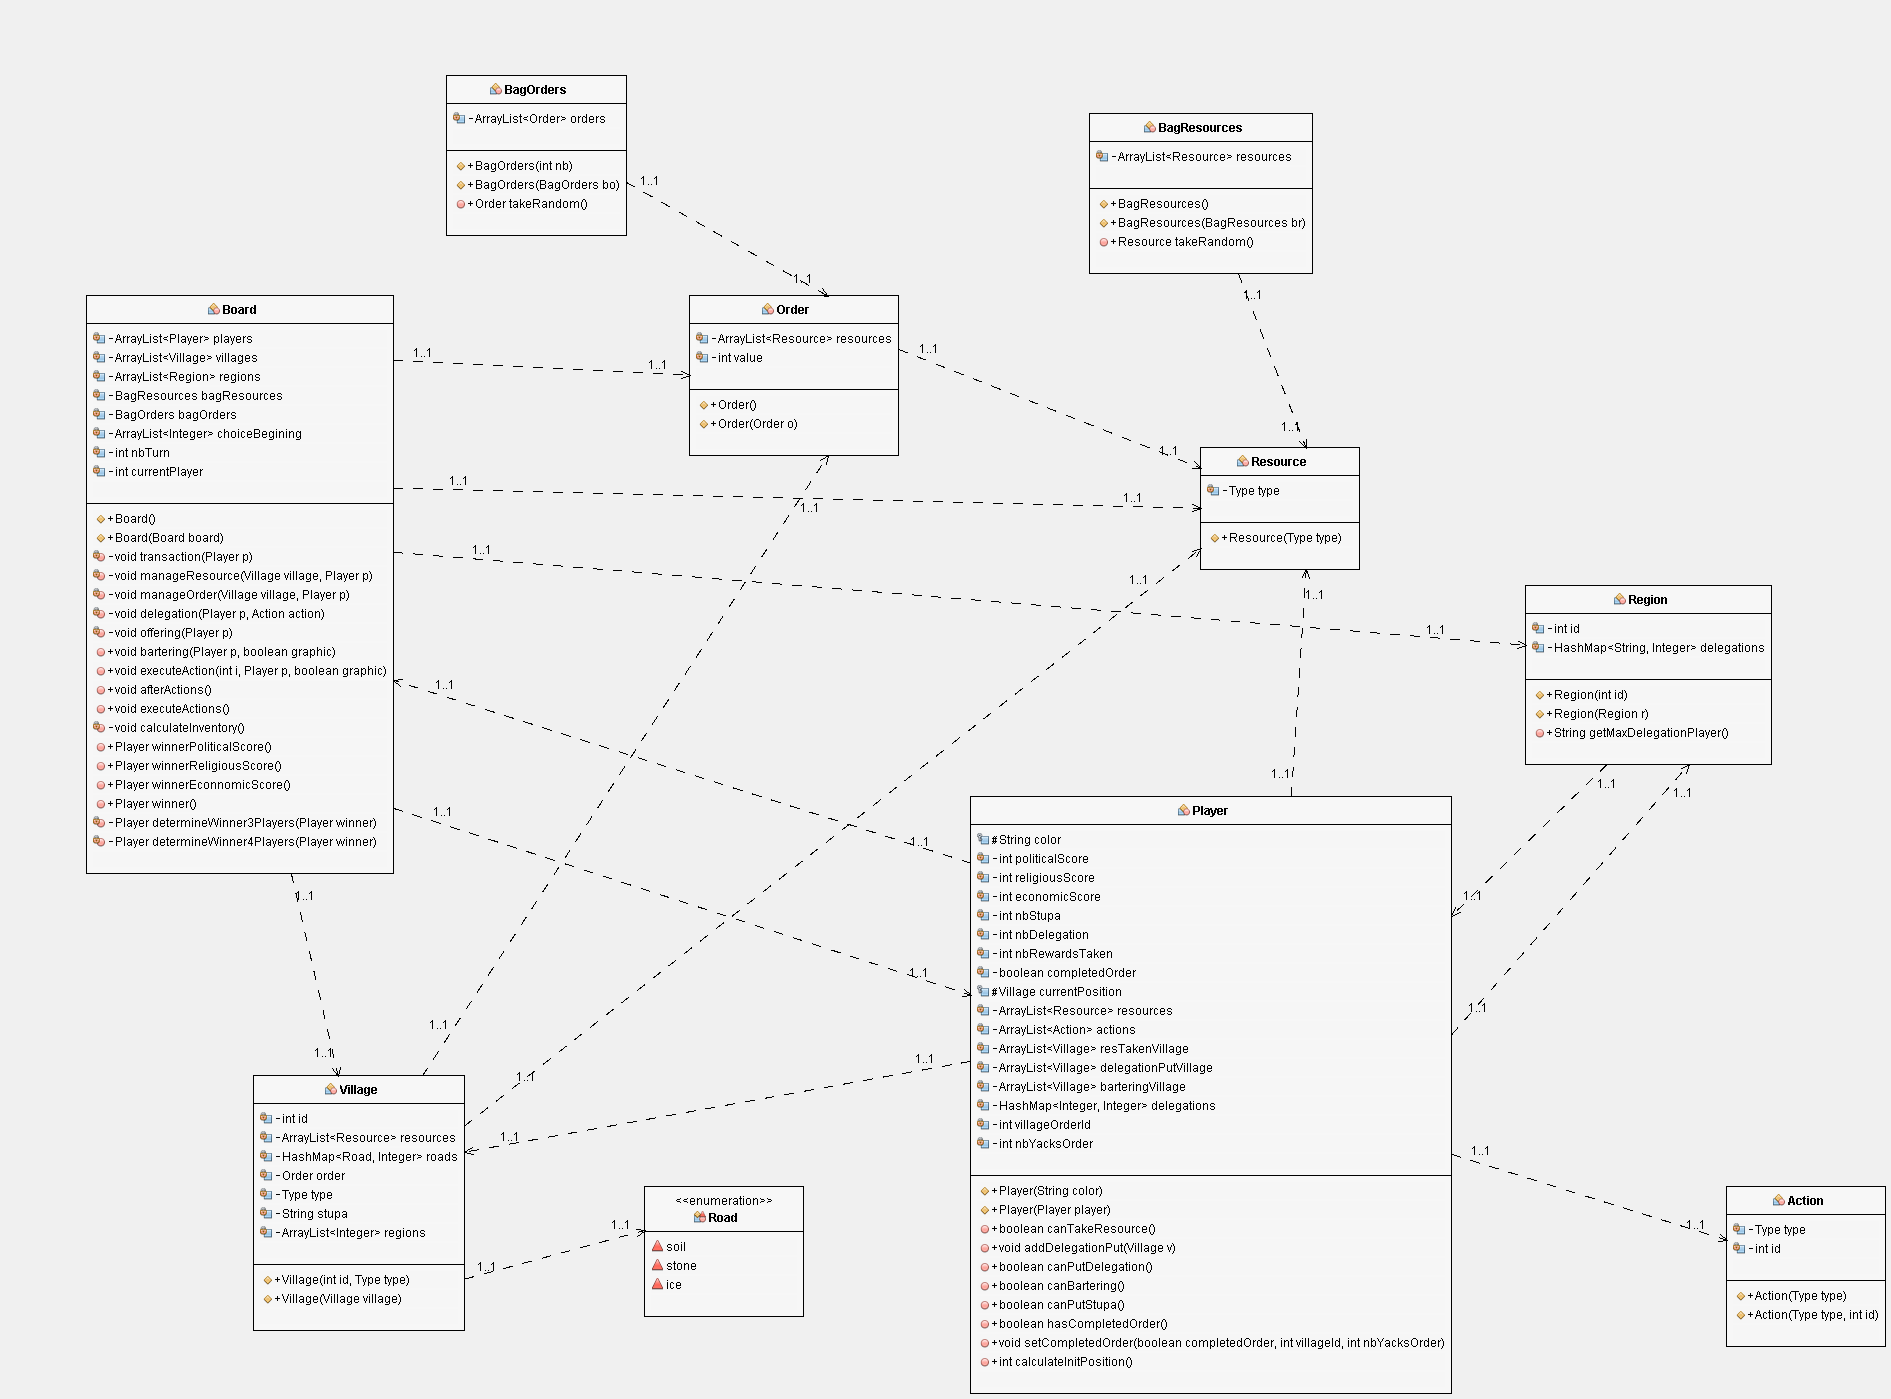
\includegraphics[width=1\linewidth]{images/UML_Himalaya_CORE_3}
	\caption{UML Moteur du jeu version 3.0 après développement}
	\label{fig:UMLCore2}
\end{figure}
\begin{figure}[h]
	\centering
	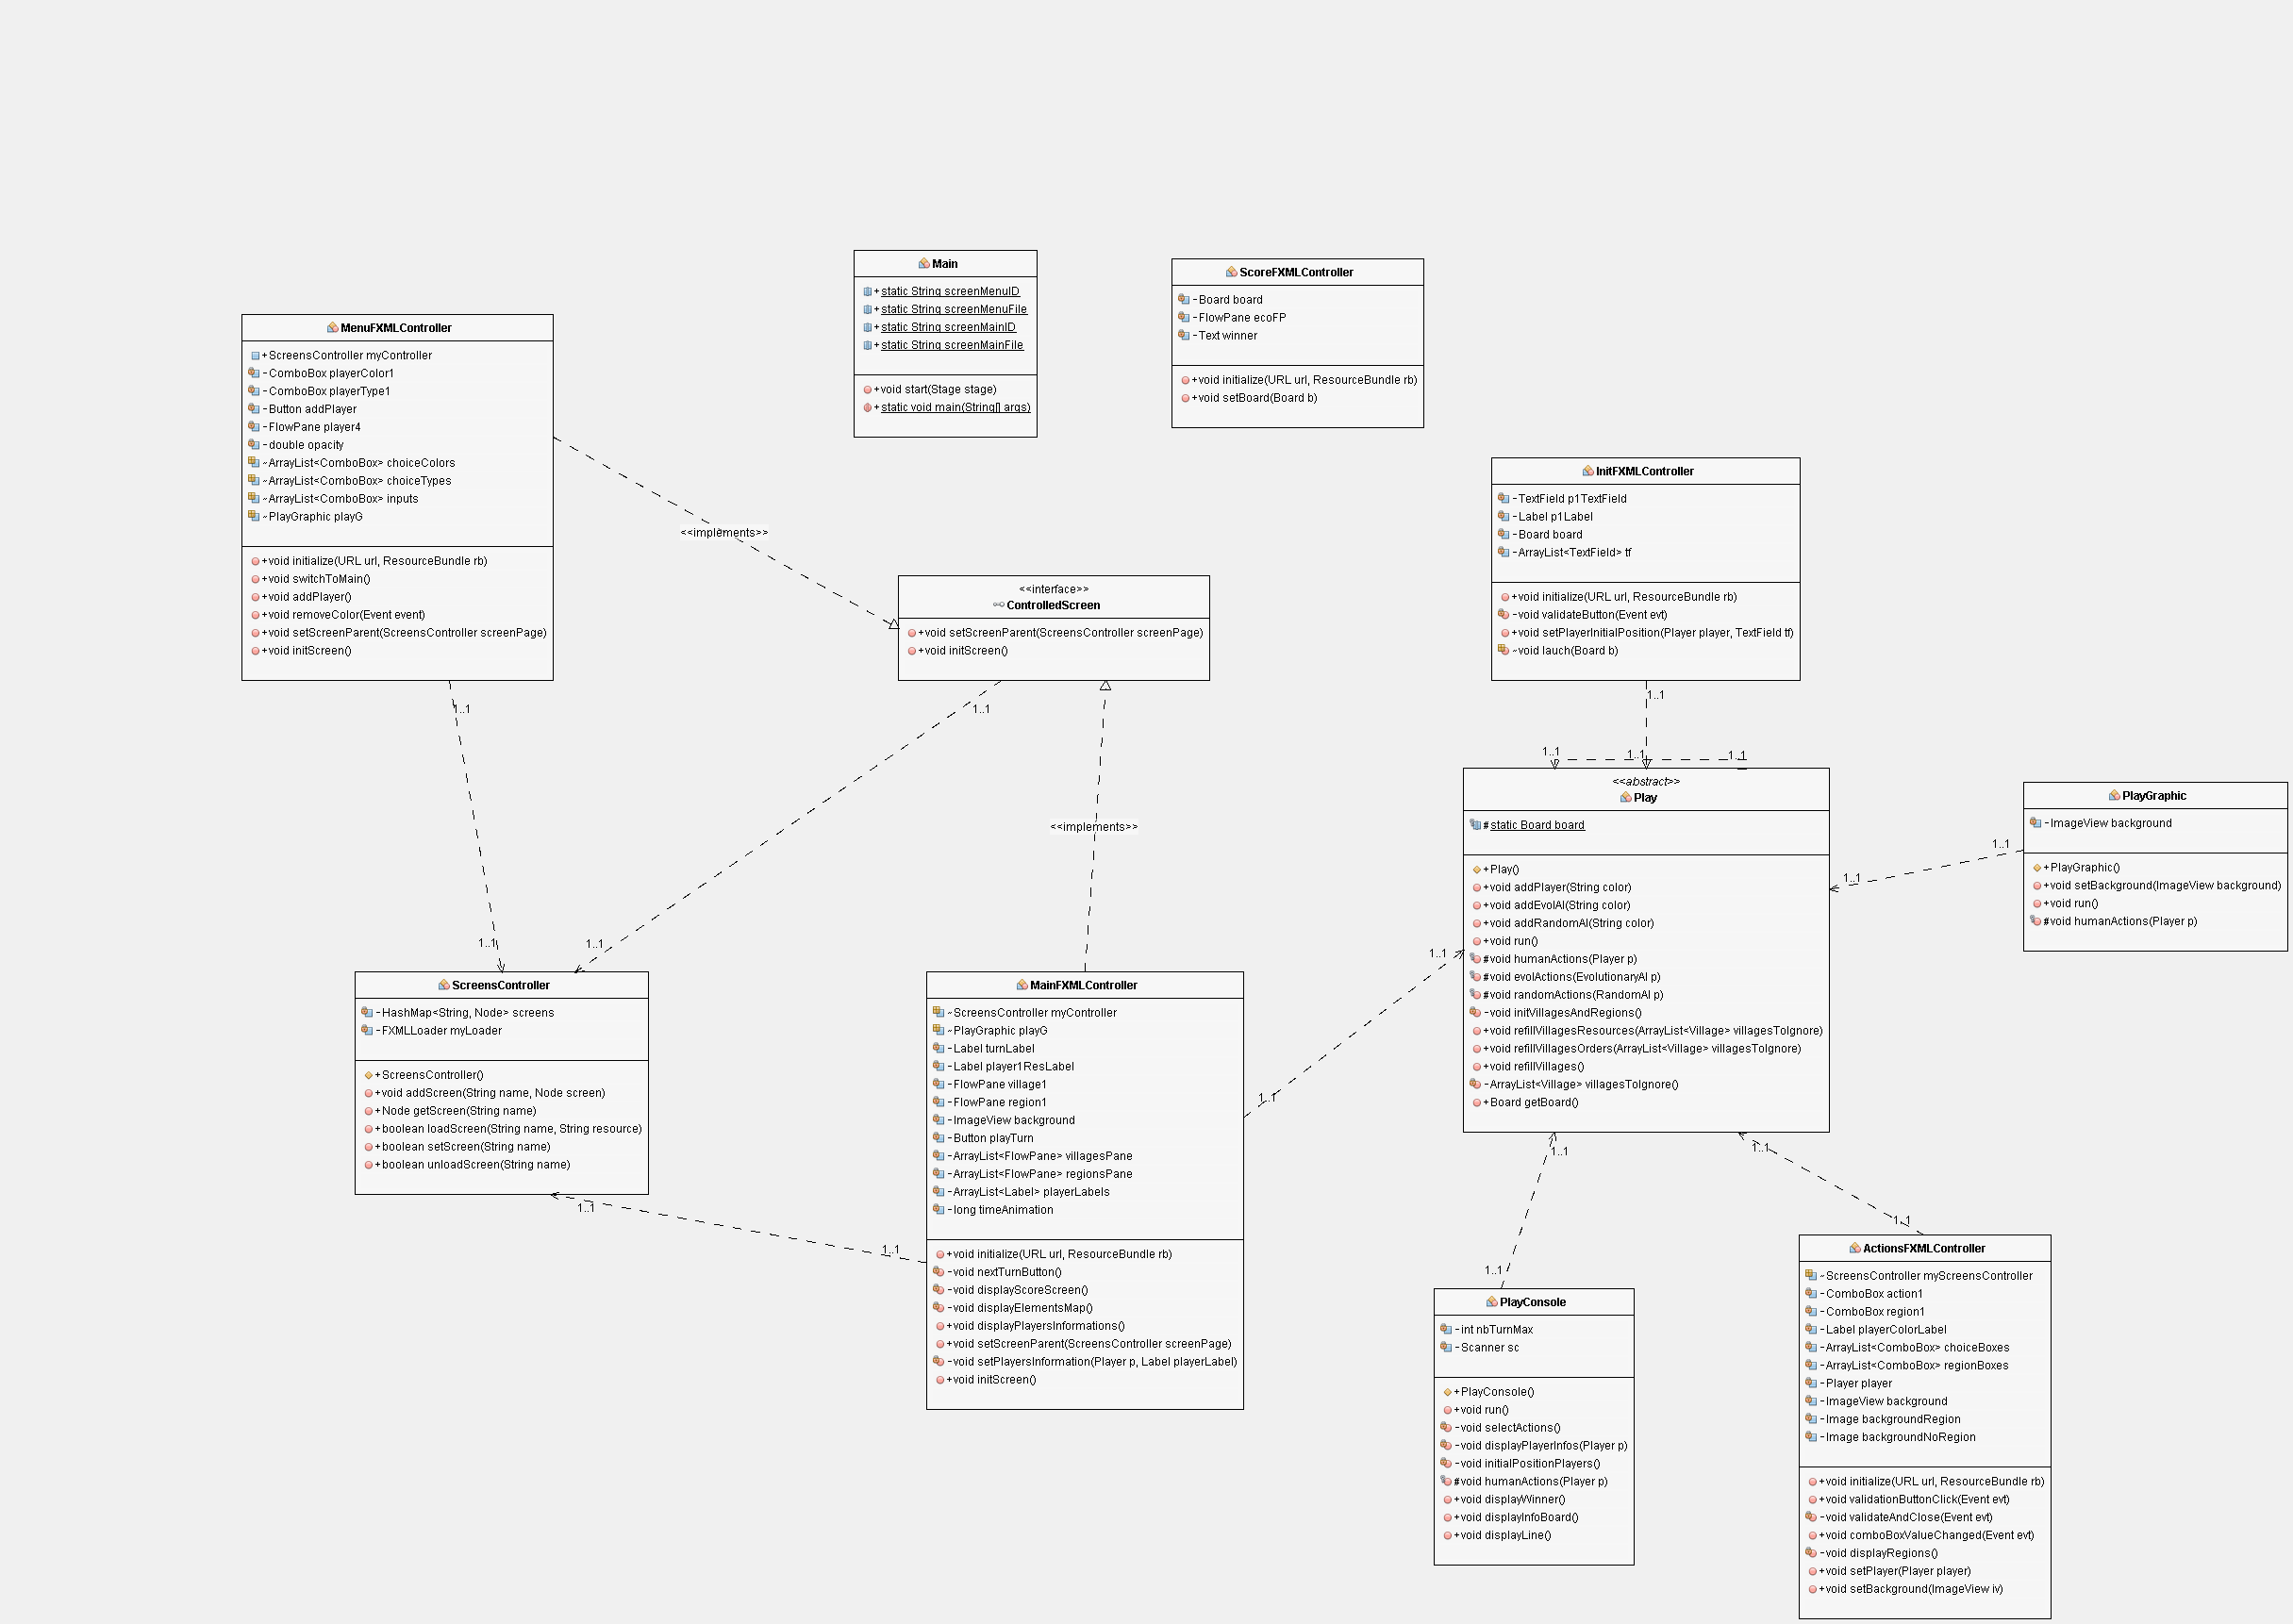
\includegraphics[width=1\linewidth]{images/UML_Himalaya_IHM_1}
	\caption{UML de l'IHM 1.0 après développement}
	\label{fig:UML_IHM}
\end{figure}
\begin{figure}[h]
	\centering
	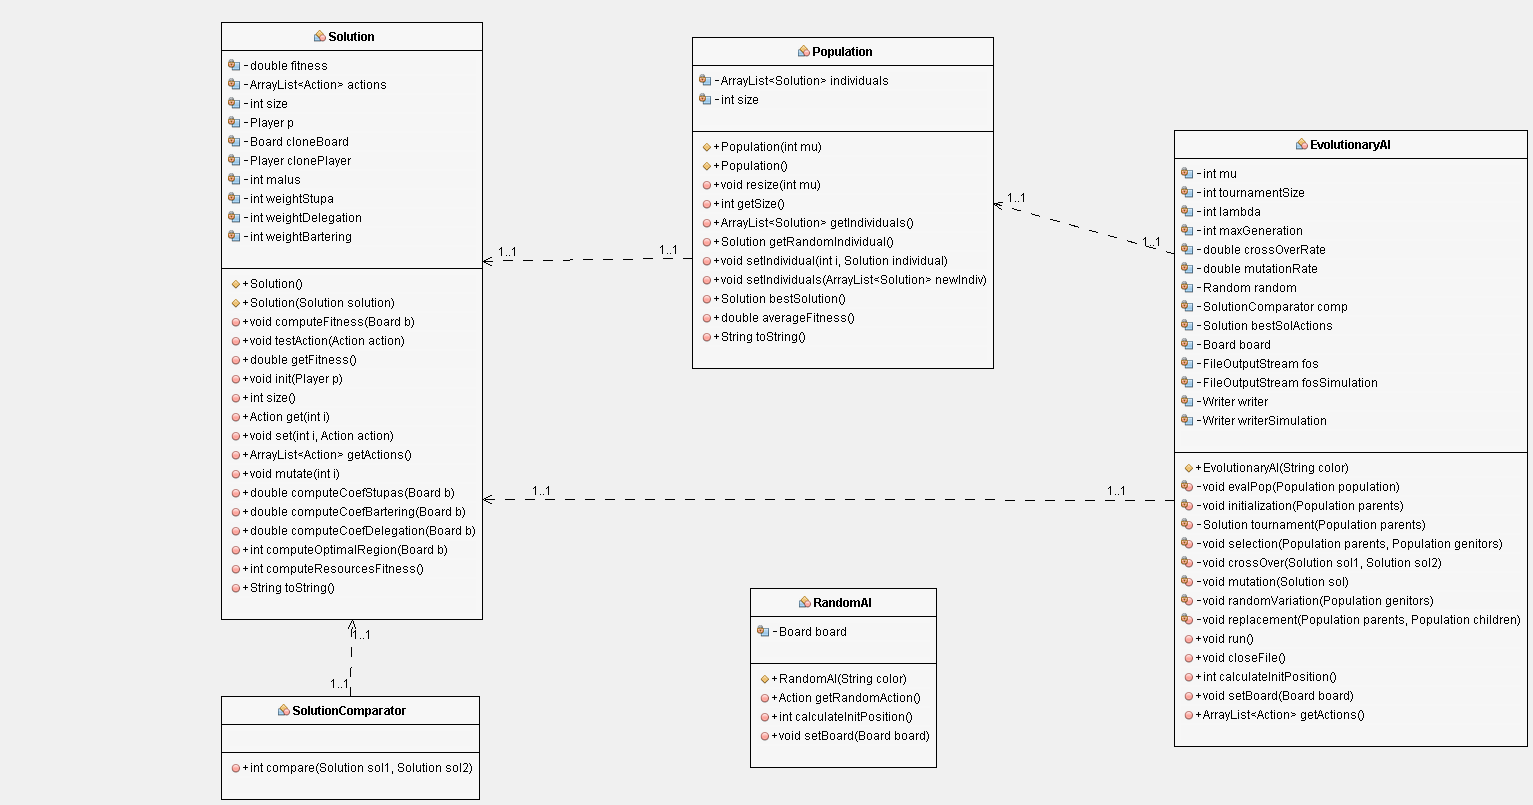
\includegraphics[width=1\linewidth]{images/UML_Himalaya_IA_1}
	\caption{UML de l'IA 1.0 après développement}
	\label{fig:UML_IA}
\end{figure}


\end{document}          
